\section{GEV models and the nested logit}\label{sec:07-nested}

The logit restricts substitution because its taste shocks are independent across products (\cref{sec:07-iia}).
A consumer who leaves product $j$ after a price increase is no more likely than anyone else to choose a
product similar to $j$. Two routes break this property while keeping the model estimable from market shares.
The first correlates the shocks of products that the analyst groups together. It leads to the generalized
extreme value family and to the nested logit. The second lets taste coefficients vary across consumers. It
leads to the random coefficients logit of \cref{ch:blp}. This section develops the first route.
\Cref{sec:07-welfare} then uses both the logit and the nested logit to measure consumer welfare.

\subsection{Generalized extreme value models}\label{sec:07-gev}

We work with an additive random utility model. Consumer $i$ obtains $u_{ij} = V_{ij} + \epsilon_{ij}$ from
alternative $j = 0, 1, \dots, J$, where $V_{ij}$ is the deterministic part of utility. Throughout this
subsection we drop the consumer index and write $V = (V_0, \dots, V_J)$ and $y_j = e^{V_j}$. The choice
probability of $j$ is $P_j(V)$. The \emph{social surplus function} is the expected maximum utility,
\begin{equation}\label{eq:07-surplus}
\mathcal{W}(V) = \E\Big[\max_{j = 0, \dots, J}\,(V_j + \epsilon_j)\Big].
\end{equation}
The logit assumes that the $\epsilon_j$ are independent type-I extreme value (Gumbel) variables.
\citet{McFadden1978} found a class of correlated distributions that keeps the closed forms of the logit. The class
is indexed by a function of $J + 1$ positive arguments.

\begin{definition}[GEV generating function]\label{def:07-gev}
A function $H : \R^{J+1}_+ \to \R_+$ is a \emph{GEV generating function} if it has the following three
properties.
\begin{enumerate}[label=(G\arabic*)]
  \item $H$ is homogeneous of degree one: $H(\lambda y) = \lambda H(y)$ for every $\lambda > 0$.
  \item $H(y) \to \infty$ as $y_j \to \infty$, for each $j$.
  \item For any $r \ge 1$ distinct indices $j_1, \dots, j_r$, the mixed partial derivative
  $\frac{\partial^r H}{\partial y_{j_1}\cdots\partial y_{j_r}}$ exists, is continuous, and is nonnegative when
  $r$ is odd and nonpositive when $r$ is even.
\end{enumerate}
\end{definition}

We write $H_j$ and $H_{jk}$ for the first and second partial derivatives of $H$. Condition (G1) produces the
closed forms below. Condition (G2) makes each marginal distribution proper. Condition (G3) makes the function in
part (i) of the next proposition a joint distribution function with a nonnegative density. The notation follows
\citet[p.~1421]{McFadden1984}, who calls the function $H$. \Cref{thm:06-gev} states and proves the first
three parts of the next result. We restate them here together with two parts that this chapter also uses, the
gradient property (iv) and the derivative formula (v).

\begin{proposition}[McFadden's GEV theorem]\label{prop:07-gev}
Let $H$ be a GEV generating function and let $y = (e^{V_0}, \dots, e^{V_J})$.
\begin{enumerate}[label=(\roman*)]
  \item $F(\epsilon_0, \dots, \epsilon_J) = \exp\big[-H(e^{-\epsilon_0}, \dots, e^{-\epsilon_J})\big]$ is the
  distribution function of a random vector whose marginals are Gumbel.
  \item If $\epsilon$ has distribution $F$, the choice probabilities are
  \begin{equation}\label{eq:07-gev-prob}
  P_j(V) = \frac{y_j H_j(y)}{H(y)} = \frac{\partial \ln H(e^{V_0}, \dots, e^{V_J})}{\partial V_j}.
  \end{equation}
  \item The maximum utility $\max_j(V_j + \epsilon_j)$ is Gumbel with location $\ln H(y)$ and scale one, so that
  \begin{equation}\label{eq:07-gev-surplus}
  \mathcal{W}(V) = \ln H(y) + \gamma_E ,
  \end{equation}
  where $\gamma_E \approx 0.5772$ is Euler's constant.
  \item (Williams, Daly and Zachary.) The social surplus function is differentiable and
  $\frac{\partial \mathcal{W}(V)}{\partial V_j} = P_j(V)$ for every $j$.
  \item For all $j$ and $k$,
  \begin{equation}\label{eq:07-gev-deriv}
  \frac{\partial P_j}{\partial V_k} = P_j\big(\indic\{j = k\} - P_k\big) + \frac{y_j y_k H_{jk}(y)}{H(y)} .
  \end{equation}
\end{enumerate}
\end{proposition}

\begin{proof}
Parts (i), (ii) and (iii) are parts (a), (b) and (c) of \cref{thm:06-gev}. Part (i) is the theorem of
\citet{McFadden1978}, and the proof of \cref{thm:06-gev} derives (ii) and (iii) from it by homogeneity. Part (iv) is
part (ii) of \cref{thm:06-wdz}, which holds for every additive random utility model. In the GEV case it also follows
by differentiating \eqref{eq:07-gev-surplus} and applying (ii). Only (v) is new.

For (v), take logs in (ii): $\ln P_j = V_j + \ln H_j(y) - \ln H(y)$. Differentiate with respect to $V_k$, using
$\frac{\partial y_k}{\partial V_k} = y_k$:
\begin{equation*}
\frac{\partial \ln P_j}{\partial V_k} = \indic\{j = k\} + \frac{y_k H_{jk}(y)}{H_j(y)} - \frac{y_k H_k(y)}{H(y)}
= \indic\{j = k\} + \frac{y_k H_{jk}(y)}{H_j(y)} - P_k .
\end{equation*}
Multiplying by $P_j = \frac{y_jH_j}{H}$ gives \eqref{eq:07-gev-deriv}.
\end{proof}

Part (v) shows what correlation buys. For $j \neq k$ the logit term $-P_jP_k$ is the cross derivative of a model
with independent shocks and the same probabilities. The second term $\frac{y_jy_kH_{jk}}{H}$ is nonpositive by
(G3). A GEV model therefore implies at least as much substitution between $j$ and $k$ as the logit at the same
choice probabilities, and $H_{jk}$ measures the excess. The formula is symmetric in $j$ and $k$, which is the
counterpart of Slutsky symmetry (\cref{cor:06-wdz}). With mean utilities $V_k = \delta_k$ and
$\delta_k = x_k\beta - \alpha p_k + \xi_k$, price derivatives follow from
$\frac{\partial s_j}{\partial p_k} = -\alpha\frac{\partial P_j}{\partial \delta_k}$.

\casehead{Two generating functions}
The logit is the case $H(y) = \sum_{j=0}^J y_j$. Its first derivatives equal one and all higher derivatives vanish,
so (ii) gives $P_j = \frac{y_j}{\sum_k y_k}$ and (v) gives the logit derivatives of \cref{prop:07-logit-derivs}.
The \emph{nested logit} groups the inside products into nests. Partition the inside products into
$G$ mutually exclusive and exhaustive nests $g = 1, \dots, G$, and place the outside good alone in nest $0$. For
a nesting parameter $\sigma$, let
\begin{equation}\label{eq:07-nl-H}
H(y) = y_0 + \sum_{g=1}^G D_g(y)^{1 - \sigma}, \qquad D_g(y) = \sum_{j \in g} y_j^{\frac{1}{1-\sigma}} .
\end{equation}

\begin{lemma}[Consistency of the nested logit]\label{lem:07-nl-gev}
The function \eqref{eq:07-nl-H} is a GEV generating function for every $\sigma \in [0, 1)$. If $\sigma < 0$ and
some nest contains two or more products, it violates (G3).
\end{lemma}

\begin{proof}
For (G1), $D_g(\lambda y) = \lambda^{\frac{1}{1-\sigma}}D_g(y)$, so $D_g(\lambda y)^{1-\sigma} = \lambda D_g(y)^{1-\sigma}$.
For (G2), if $y_j \to \infty$ with $j \in g$, then $D_g \to \infty$ and $D_g^{1-\sigma} \to \infty$ because
$1 - \sigma > 0$. The outside good enters linearly.

For (G3), a mixed partial derivative over indices from two different nests is zero, which satisfies the weak sign
condition. Take distinct indices $j_1, \dots, j_r$ in the same nest $g$. Write $\varphi(D) = D^{1-\sigma}$ and
$a_j = \frac{\partial D_g}{\partial y_j} = \frac{1}{1-\sigma}y_j^{\frac{\sigma}{1-\sigma}} \ge 0$. Each $a_j$ depends on
$y_j$ alone, so the chain rule gives
\begin{equation*}
\frac{\partial^r H}{\partial y_{j_1}\cdots\partial y_{j_r}} = \varphi^{(r)}(D_g)\prod_{m=1}^r a_{j_m} .
\end{equation*}
The successive derivatives of $\varphi$ are $\varphi'(D) = (1-\sigma)D^{-\sigma}$,
$\varphi''(D) = -\sigma(1-\sigma)D^{-\sigma-1}$, $\varphi'''(D) = \sigma(\sigma+1)(1-\sigma)D^{-\sigma-2}$, and in general
\begin{equation*}
\varphi^{(r)}(D) = (-1)^{r-1}(1-\sigma)\prod_{m=0}^{r-2}(\sigma + m)\,D^{1-\sigma-r}, \qquad r \ge 2 .
\end{equation*}
For $\sigma \in [0, 1)$ every factor in the product is nonnegative, so the sign is $(-1)^{r-1}$, as (G3) requires.
If $\sigma < 0$, then $\varphi''(D) > 0$ and the second mixed derivative of two products in the same nest is
positive.
\end{proof}

The parameter range has an empirical counterpart. \citet[pp.~1425--1426]{McFadden1984} notes that estimates of
the nesting parameters outside the unit interval violate the ranking of cross elasticities implied by the tree,
and may indicate a misspecified tree. In the notation of \citet{BorschSupan1990}, our $1 - \sigma$ is the
dissimilarity parameter. He shows that values with $\sigma < 0$ can still be consistent with utility maximization
on a restricted region of mean utilities (Section~4 and Theorem~1, pp.~377--381). By Theorem~1, it suffices that
the mixed partial derivatives of the choice probabilities be nonnegative on that region. In the two-level model
this requires the choice probabilities of the nests to be large enough (Theorem~2, p.~385). With two nests of two
alternatives each and a common $\sigma < -1$, these requirements conflict and no such region exists (p.~385).
Applied work treats $\sigma \in [0, 1)$ as the admissible range. The next two subsections derive the nested logit a second way,
from an explicit utility model.

\subsection{The nested logit model}\label{sec:07-nl-model}

The nested logit relaxes IIA by grouping products. Within a nest, consumers substitute as in the logit. Products in
different nests have less in common, so they are weaker substitutes. The idea parallels the grouping of goods in
multi-stage budgeting (\cref{ch:aids}), and the same analyst judgment determines the groups.

\begin{assumption}[Nested logit]\label{asm:07-nl}
The inside products of market $t$ are partitioned into nests $g = 1, \dots, G$, and the outside good forms nest
$0$ by itself. The utility of consumer $i$ from product $j$ in nest $g$ is
\begin{equation}\label{eq:07-nl-utility}
u_{ij} = \delta_j + \zeta_{ig} + (1 - \sigma)\epsilon_{ij}, \qquad \delta_j = x_j\beta - \alpha p_j + \xi_j ,
\end{equation}
and the utility of the outside good is a standard Gumbel variable $\epsilon_{i0}$. The shocks $\epsilon_{ij}$ are
i.i.d.\ standard Gumbel. The nest tastes $\zeta_{ig}$ are i.i.d.\ across consumers and nests with the distribution
$C(\sigma)$ of \cref{lem:07-cardell}, and they are independent of the $\epsilon_{ij}$. The nesting parameter
satisfies $0 \le \sigma < 1$.
\end{assumption}

The term $\zeta_{ig}$ is common to all products in nest $g$ for consumer $i$. A consumer with a high draw likes
every product of the nest, so the utilities of products in the same nest are positively correlated.
\citet[p.~252]{Berry1994} points out that \eqref{eq:07-nl-utility} is a random coefficients model. Let $d_{jh}$
equal one if $j \in h$. Then $\zeta_{ig} = \sum_h d_{jh}\zeta_{ih}$ for $j \in g$, so the nest taste is a random
coefficient on the nest dummies, with a distribution tied to $\sigma$. Unlike the full random coefficients model, correlation can depend only on
groupings fixed before estimation, never on continuous characteristics. \Citet[p.~524]{Nevo2000a} makes the same
point, and \citet{Cardell1997} shows that the two descriptions of the nested logit are equivalent. The
distribution of $\zeta_{ig}$ is chosen so that the composite shock remains Gumbel.

\begin{lemma}[\citealp{Cardell1997}]\label{lem:07-cardell}
For every $\sigma \in [0, 1)$ there is a unique distribution $C(\sigma)$ with the following property. If
$\zeta \sim C(\sigma)$ and $\epsilon$ is a standard Gumbel variable independent of $\zeta$, then
$\zeta + (1 - \sigma)\epsilon$ is a standard Gumbel variable. Equivalently, the random variable
$X = e^{\frac{\zeta}{1-\sigma}}$ satisfies
\begin{equation}\label{eq:07-cardell-laplace}
\E\big[e^{-cX}\big] = \exp\big(-c^{1-\sigma}\big) \qquad \text{for every } c > 0 .
\end{equation}
\end{lemma}

We do not prove existence, which \citet{Cardell1997} establishes along with the density of $\zeta$. The
equivalence is a short computation. Conditioning on $\zeta$,
\begin{equation*}
\Pr\big(\zeta + (1-\sigma)\epsilon \le t\big) = \E\Big[\exp\Big(-e^{-\frac{t - \zeta}{1-\sigma}}\Big)\Big]
= \E\big[e^{-cX}\big], \qquad c = e^{-\frac{t}{1-\sigma}} .
\end{equation*}
The standard Gumbel distribution function is $\exp(-e^{-t}) = \exp(-c^{1-\sigma})$, which gives
\eqref{eq:07-cardell-laplace}. A Laplace transform determines a distribution, which explains uniqueness. The
function $c \mapsto \exp(-c^{a})$ with $0 < a \le 1$ is the Laplace transform of the positive stable law of index
$a$ \citep{Feller1971}. So $\zeta$ is $(1-\sigma)$ times the logarithm of a positive stable variable of index
$1 - \sigma$. At $\sigma = 0$ the stable variable equals one and $\zeta = 0$.

\begin{proposition}[Nested logit shares]\label{prop:07-nl-shares}
Under \cref{asm:07-nl}, define the inclusive sum of nest $g$ as
$D_g = \sum_{k \in g} e^{\frac{\delta_k}{1-\sigma}}$. Then the within-nest share, the nest share, the product share
and the outside share are
\begin{equation}\label{eq:07-nl-share}
s_{j \mid g} = \frac{e^{\frac{\delta_j}{1-\sigma}}}{D_g}, \qquad
s_g = \frac{D_g^{1-\sigma}}{1 + \sum_{h=1}^G D_h^{1-\sigma}}, \qquad
s_j = s_{j \mid g}\,s_g, \qquad
s_0 = \frac{1}{1 + \sum_{h=1}^G D_h^{1-\sigma}} .
\end{equation}
The composite shocks $\zeta_{ig} + (1-\sigma)\epsilon_{ij}$ have the GEV distribution generated by
\eqref{eq:07-nl-H}.
\end{proposition}

\begin{proof}
We give two derivations. The first uses \cref{prop:07-gev}. The second builds the shares nest by nest.

\emph{GEV derivation.} Fix a nest $g$ and numbers $t_j$ for $j \in g$. Conditioning on $\zeta_{ig}$ and using the
independence of the $\epsilon_{ij}$,
\begin{equation*}
\Pr\big(\zeta_{ig} + (1-\sigma)\epsilon_{ij} \le t_j \text{ for all } j \in g\big)
= \E\Big[\prod_{j\in g}\exp\Big(-e^{-\frac{t_j - \zeta_{ig}}{1-\sigma}}\Big)\Big]
= \E\Big[\exp\Big(-X\sum_{j \in g}e^{-\frac{t_j}{1-\sigma}}\Big)\Big],
\end{equation*}
with $X = e^{\frac{\zeta_{ig}}{1-\sigma}}$. By \eqref{eq:07-cardell-laplace} the last expression equals
$\exp\big[-\big(\sum_{j\in g}e^{-\frac{t_j}{1-\sigma}}\big)^{1-\sigma}\big]$. Nests are independent and the outside
shock contributes $\exp(-e^{-t_0})$. The joint distribution function is therefore $\exp[-H(e^{-t_0}, \dots,
e^{-t_J})]$ with $H$ from \eqref{eq:07-nl-H}. Apply \eqref{eq:07-gev-prob} with $y_j = e^{\delta_j}$ and
$y_0 = 1$. For $j \in g$,
\begin{equation*}
H_j(y) = (1-\sigma)D_g^{-\sigma}\cdot\frac{1}{1-\sigma}y_j^{\frac{\sigma}{1-\sigma}} = D_g^{-\sigma}y_j^{\frac{\sigma}{1-\sigma}},
\qquad y_jH_j(y) = D_g^{-\sigma}e^{\frac{\delta_j}{1-\sigma}} .
\end{equation*}
Dividing by $H(y) = 1 + \sum_h D_h^{1-\sigma}$,
\begin{equation*}
s_j = \frac{e^{\frac{\delta_j}{1-\sigma}}D_g^{-\sigma}}{1 + \sum_h D_h^{1-\sigma}}
= \frac{e^{\frac{\delta_j}{1-\sigma}}}{D_g}\cdot\frac{D_g^{1-\sigma}}{1 + \sum_h D_h^{1-\sigma}} .
\end{equation*}
The two factors are $s_{j \mid g}$ and $s_g$. For the outside good, $y_0H_0 = 1$ gives $s_0$.

\emph{Sequential derivation.} Within nest $g$ the term $\zeta_{ig}$ is common to all products, so it does not
affect which product of the nest is best. Dividing utilities by $1 - \sigma$ shows that the best product in the
nest maximizes $\frac{\delta_j}{1-\sigma} + \epsilon_{ij}$. This is a logit with mean utilities
$\frac{\delta_j}{1-\sigma}$, so $s_{j \mid g} = \frac{e^{\frac{\delta_j}{1-\sigma}}}{D_g}$ by \eqref{eq:07-logit-share}
without the outside good. By max-stability of the Gumbel (\cref{lem:06-maxstable}),
\begin{equation*}
\max_{j\in g}\big(\delta_j + (1-\sigma)\epsilon_{ij}\big) = (1-\sigma)\max_{j\in g}\Big(\frac{\delta_j}{1-\sigma} + \epsilon_{ij}\Big)
= I_g + (1-\sigma)\tilde\epsilon_{ig}, \qquad I_g = (1-\sigma)\ln D_g ,
\end{equation*}
where $\tilde\epsilon_{ig}$ is standard Gumbel and independent across nests. The best utility available in nest
$g$ is $I_g + \zeta_{ig} + (1-\sigma)\tilde\epsilon_{ig}$. By \cref{lem:07-cardell}, the composite term
$\zeta_{ig} + (1-\sigma)\tilde\epsilon_{ig}$ is standard Gumbel, independent across nests and of $\epsilon_{i0}$. The
choice of nest is therefore a logit with mean utilities $I_g$ and $0$ for the outside good:
\begin{equation*}
s_g = \frac{e^{I_g}}{1 + \sum_h e^{I_h}} = \frac{D_g^{1-\sigma}}{1 + \sum_h D_h^{1-\sigma}} .
\end{equation*}
Finally, the identity of the best product within a nest is independent of the value of the within-nest maximum
(\cref{eq:06-maxindep}). The event that $j$ is best within $g$ is therefore independent of the event that nest
$g$ wins, and $s_j = s_{j \mid g}s_g$.
\end{proof}

The quantity $I_g = (1 - \sigma)\ln D_g$ is the \emph{inclusive value} of nest $g$. It is the location of the best
utility the nest offers before the nest taste is added. It summarizes the whole nest in one number, much as a group
price index summarizes a group in multi-stage budgeting. Let $\bar\delta_g = \max_{k \in g}\delta_k$. Because
$D_g \ge e^{\frac{\bar\delta_g}{1-\sigma}}$, the inclusive value is at least $\bar\delta_g$. With $J_g$ identical products of mean utility
$\delta$, it equals $\delta + (1-\sigma)\ln J_g$, so a nest gains value from variety at rate $1 - \sigma$.

\casehead{Correlation within nests}
The composite shock of product $j \in g$ is $\zeta_{ig} + (1-\sigma)\epsilon_{ij}$, a standard Gumbel variable
with variance $\frac{\pi^2}{6}$. The term $(1-\sigma)\epsilon_{ij}$ has variance $(1-\sigma)^2\frac{\pi^2}{6}$.
Since $\zeta_{ig}$ and $\epsilon_{ij}$ are independent,
\begin{equation*}
\Var(\zeta_{ig}) = \frac{\pi^2}{6} - (1-\sigma)^2\frac{\pi^2}{6} = \big[1 - (1-\sigma)^2\big]\frac{\pi^2}{6} .
\end{equation*}
For two products $j \neq k$ in the same nest, the only common component is $\zeta_{ig}$, so
$\Cov(u_{ij}, u_{ik}) = \Var(\zeta_{ig})$. Dividing by the common variance $\frac{\pi^2}{6}$,
\begin{equation}\label{eq:07-nl-corr}
\Corr(u_{ij}, u_{ik}) = 1 - (1-\sigma)^2 = \sigma(2 - \sigma), \qquad j, k \in g, \; j \neq k .
\end{equation}
Utilities of products in different nests are uncorrelated. The correlation rises from zero at $\sigma = 0$ to one as
$\sigma \to 1$. At $\sigma = 0.5$ it is $0.75$.

\casehead{The two limits}
At $\sigma = 0$ the nest tastes vanish, $D_g^{1-\sigma} = \sum_{k \in g}e^{\delta_k}$, and \eqref{eq:07-nl-share}
is the logit share \eqref{eq:07-logit-share}. The limit $\sigma \to 1$ answers the question of which products
consumers buy when utilities within a nest become perfectly correlated. Let $r_g$ be the number of products in
$g$ whose mean utility equals $\bar\delta_g$. Then
\begin{equation*}
s_{j \mid g} = \frac{1}{\sum_{k \in g}e^{\frac{\delta_k - \delta_j}{1-\sigma}}} \longrightarrow
\begin{cases}
\frac{1}{r_g} & \text{if } \delta_j = \bar\delta_g, \\
0 & \text{otherwise},
\end{cases}
\end{equation*}
because every exponent $\frac{\delta_k - \delta_j}{1 - \sigma}$ with $\delta_k > \delta_j$ diverges to $+\infty$. For the nest
level,
\begin{equation*}
D_g^{1-\sigma} = e^{\bar\delta_g}\Big(\sum_{k\in g}e^{\frac{\delta_k - \bar\delta_g}{1-\sigma}}\Big)^{1-\sigma}
\longrightarrow e^{\bar\delta_g}\cdot\lim_{\sigma\to 1} r_g^{1-\sigma} = e^{\bar\delta_g} ,
\end{equation*}
since the sum converges to $r_g$. Nest shares converge to $\frac{e^{\bar\delta_g}}{1 + \sum_h e^{\bar\delta_h}}$.
In the limit only the product with the highest mean utility in each nest is bought, and each nest behaves like a
single product with that mean utility. Products within a nest become perfect substitutes, while nests remain logit
substitutes for one another. \Cref{fig:07-nl-tree} shows the one-level tree and the two-level tree of
\cref{sec:07-nl-twolevel}.

\begin{figure}[htbp]
\centering
\begin{subfigure}[b]{0.49\textwidth}
\centering
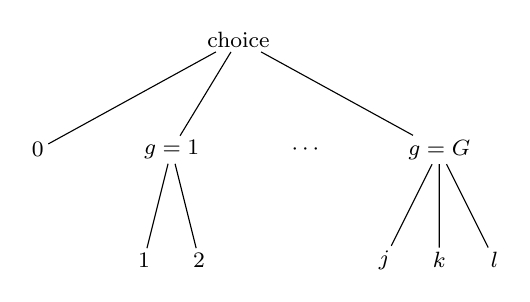
\begin{tikzpicture}[font=\footnotesize, level distance=14mm,
  level 1/.style={sibling distance=17mm}, level 2/.style={sibling distance=7mm},
  every node/.style={inner sep=1.5pt}]
\node (root) {choice}
  child {node {$0$}}
  child {node {$g = 1$}
    child {node {$1$}}
    child {node {$2$}}}
  child {node {$\cdots$} edge from parent[draw=none]}
  child {node {$g = G$}
    child {node {$j$}}
    child {node {$k$}}
    child {node {$l$}}};
\end{tikzpicture}
\caption{One level}
\end{subfigure}\hfill
\begin{subfigure}[b]{0.49\textwidth}
\centering
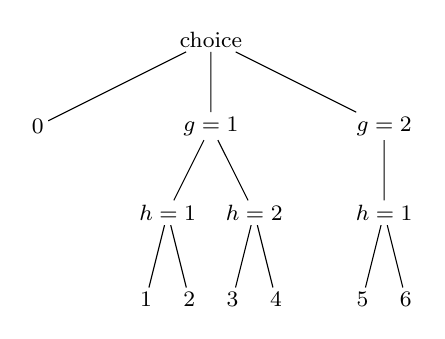
\begin{tikzpicture}[font=\footnotesize, level distance=11mm,
  level 1/.style={sibling distance=22mm}, level 2/.style={sibling distance=11mm},
  level 3/.style={sibling distance=5.5mm},
  every node/.style={inner sep=1.5pt}]
\node {choice}
  child {node {$0$}}
  child {node {$g = 1$}
    child {node {$h = 1$}
      child {node {$1$}}
      child {node {$2$}}}
    child {node {$h = 2$}
      child {node {$3$}}
      child {node {$4$}}}}
  child {node {$g = 2$}
    child {node {$h = 1$}
      child {node {$5$}}
      child {node {$6$}}}};
\end{tikzpicture}
\caption{Two levels}
\end{subfigure}
\caption{Nesting trees. In panel (a) the outside good $0$ is alone in its nest and the inside products are grouped
into nests $g = 1, \dots, G$. The nest choice is a logit in the inclusive values $I_g = (1-\sigma)\ln D_g$, and the
choice within a nest is a logit with scale $1 - \sigma$. In panel (b) each group $g$ is split into subgroups $h$,
with within-subgroup parameter $\sigma_1$ and within-group parameter $\sigma_2 \le \sigma_1$.}
\label{fig:07-nl-tree}
\end{figure}

\subsection{Substitution patterns}\label{sec:07-nl-substitution}

All substitution patterns follow from one derivative. Taking logs in \eqref{eq:07-nl-share},
\begin{align*}
\ln s_j &= \ln s_{j \mid g} + \ln s_g \\
&= \frac{\delta_j}{1-\sigma} - \ln D_g + (1-\sigma)\ln D_g - \ln\Big(1 + \sum_h D_h^{1-\sigma}\Big) \\
&= \frac{\delta_j}{1-\sigma} - \sigma\ln D_g - \ln\Big(1 + \sum_h D_h^{1-\sigma}\Big) .
\end{align*}
Differentiate each term with respect to $\delta_k$. The first term gives $\frac{\indic\{j = k\}}{1-\sigma}$. For the
second, $\frac{\partial \ln D_g}{\partial \delta_k} = \frac{1}{1-\sigma}s_{k \mid g}$ if $k \in g$ and zero otherwise.
For the third, if $k$ belongs to nest $h$,
\begin{equation*}
\frac{\partial}{\partial \delta_k}\ln\Big(1 + \sum_{h'} D_{h'}^{1-\sigma}\Big)
= \frac{(1-\sigma)D_h^{-\sigma}\cdot\frac{1}{1-\sigma}e^{\frac{\delta_k}{1-\sigma}}}{1 + \sum_{h'}D_{h'}^{1-\sigma}}
= s_{k \mid h}\,s_h = s_k .
\end{equation*}
Collecting terms,
\begin{equation}\label{eq:07-nl-dlns}
\frac{\partial \ln s_j}{\partial \delta_k} = \frac{\indic\{j = k\}}{1-\sigma} - \frac{\sigma}{1-\sigma}\,s_{k \mid g}\,\indic\{k \in g\} - s_k ,
\qquad j \in g .
\end{equation}
The same expression follows from \eqref{eq:07-gev-deriv} with the generating function \eqref{eq:07-nl-H}. Since
$\frac{\partial \delta_k}{\partial p_k} = -\alpha$, the price derivatives are
\begin{align}
\frac{\partial s_j}{\partial p_j} &= -\alpha s_j\Big[\frac{1}{1-\sigma} - \frac{\sigma}{1-\sigma}s_{j \mid g} - s_j\Big], \label{eq:07-nl-own}\\
\frac{\partial s_j}{\partial p_k} &= \alpha s_j\Big[\frac{\sigma}{1-\sigma}s_{k \mid g} + s_k\Big], \qquad k \in g,\; k \neq j, \label{eq:07-nl-cross-in}\\
\frac{\partial s_j}{\partial p_k} &= \alpha s_j s_k, \qquad k \notin g . \label{eq:07-nl-cross-out}
\end{align}
The bracket in \eqref{eq:07-nl-own} equals $\frac{1 - \sigma s_{j \mid g} - (1-\sigma)s_j}{1-\sigma}$, which is positive
because $s_{j \mid g} \le 1$ and $s_j < 1$. Multiplying by $\frac{p_j}{s_j}$ or $\frac{p_k}{s_j}$ gives the elasticities.
With the own elasticity written as a positive number,
\begin{equation}\label{eq:07-nl-elast}
\varepsilon_j = \alpha p_j\Big[\frac{1}{1-\sigma} - \frac{\sigma}{1-\sigma}s_{j \mid g} - s_j\Big], \qquad
\varepsilon_{jk} =
\begin{cases}
\alpha p_k\Big[\frac{\sigma}{1-\sigma}s_{k \mid g} + s_k\Big], & k \in g, \\[4pt]
\alpha p_k s_k, & k \notin g .
\end{cases}
\end{equation}

These formulas have four implications.
\begin{enumerate}[label=(\alph*)]
  \item Within a nest, substitution is proportional to shares. The cross elasticity $\varepsilon_{jk}$ for
  $k \in g$ depends on $k$ alone, so a rise in $p_k$ raises the shares of all of $k$'s nest-mates in the same
  proportion. Equivalently, $\frac{s_j}{s_l} = e^{\frac{\delta_j - \delta_l}{1-\sigma}}$ for $j, l \in g$, so IIA holds
  within each nest.
  \item Across nests, substitution is also proportional to shares. A rise in $p_k$ raises the shares of all
  products outside $k$'s nest, and of the outside good, by the same proportion $\alpha s_k\,\dd p_k$, exactly as in
  the logit.
  \item The same-nest cross elasticity exceeds the cross elasticity for products in other nests by
  $\alpha p_k\frac{\sigma}{1-\sigma}s_{k \mid g}$. This is the extra substitution among similar products that the
  logit lacks.
  \item IIA fails between products in different nests. For $j \in g$ and $l \in h \neq g$,
  $\frac{s_j}{s_l} = e^{\frac{\delta_j - \delta_l}{1-\sigma}}\big(\frac{D_h}{D_g}\big)^{\sigma}$ depends on every product of
  the two nests.
\end{enumerate}
The own elasticity keeps the main defect of the logit. For small shares it is close to
$\frac{\alpha p_j}{1-\sigma}(1 - \sigma s_{j \mid g})$, which rises almost in proportion to price. As
\citet[p.~524]{Nevo2000a} puts it, the nested logit ``does not help with the problem of own-price elasticities''.

\casehead{Diversion ratios}
Recall from \cref{sec:07-logit-elasticities} that the diversion ratio $D_{jk} = -\frac{\partial s_k}{\partial
p_j}\big(\frac{\partial s_j}{\partial p_j}\big)^{-1}$ is the fraction of the sales that $j$ loses after a small price
increase that go to $k$. For $k$ in the same nest as $j$,
\eqref{eq:07-nl-cross-in} with the roles of $j$ and $k$ exchanged gives
$\frac{\partial s_k}{\partial p_j} = \alpha s_k\big[\frac{\sigma}{1-\sigma}s_{j \mid g} + s_j\big]$. Because
$s_ks_{j \mid g} = s_{k \mid g}s_gs_{j \mid g} = s_js_{k \mid g}$, this equals
$\alpha s_j\big[\frac{\sigma}{1-\sigma}s_{k \mid g} + s_k\big]$. Dividing by minus \eqref{eq:07-nl-own} and multiplying
numerator and denominator by $1 - \sigma$,
\begin{equation}\label{eq:07-nl-diversion}
D_{jk} =
\begin{cases}
\frac{\sigma s_{k \mid g} + (1-\sigma)s_k}{1 - \sigma s_{j \mid g} - (1-\sigma)s_j}, & k \in g, \\[6pt]
\frac{(1-\sigma)s_k}{1 - \sigma s_{j \mid g} - (1-\sigma)s_j}, & k \notin g .
\end{cases}
\end{equation}
The diversion to the outside good, $D_{j0}$, has the second form with $s_0$ in place of $s_k$. The ratios sum to one.
Summing the numerators over $k \in g$ with $k \neq j$, over the other nests, and over the outside good gives
\begin{equation*}
\sigma(1 - s_{j \mid g}) + (1-\sigma)(1 - s_j) = 1 - \sigma s_{j \mid g} - (1-\sigma)s_j ,
\end{equation*}
which is the denominator. At $\sigma = 0$ every ratio reduces to the logit value $\frac{s_k}{1-s_j}$. Now let
$\sigma \to 1$ with the shares held fixed and $s_{j \mid g} < 1$. Then all diversion stays within the nest, in
proportion to within-nest shares. The condition on $s_{j \mid g}$ matters. Writing the denominator as
$\sigma(1 - s_{j \mid g}) + (1-\sigma)(1 - s_j)$,
\begin{equation*}
D_{j0} = \frac{(1-\sigma)s_0}{\sigma(1 - s_{j \mid g}) + (1-\sigma)(1 - s_j)} ,
\end{equation*}
which vanishes only if $\frac{1 - s_{j \mid g}}{1-\sigma}$ grows without bound. A product alone in its nest has
$s_{j \mid g} = 1$, so $D_{j0} = \frac{s_0}{1 - s_j}$ for every $\sigma$. The limit also fails when mean utilities,
rather than shares, are held fixed and $j$ is the unique best product in its nest. Then $1 - s_{j \mid g}$ falls
exponentially in $\frac{1}{1-\sigma}$, and $D_{j0}$ tends to $\frac{s_0}{1 - s_j}$ at the limiting shares.
\Cref{tab:07-nl-formulas} collects the formulas of this section and the next three subsections.

\begin{table}[htbp]
\centering
\caption{Logit and nested logit formulas}\label{tab:07-nl-formulas}
\small
\renewcommand{\arraystretch}{1.8}
\begin{tabular}{@{}lll@{}}
\toprule
Object & Logit & Nested logit ($j \in g$) \\
\midrule
Share $s_j$ & $\displaystyle \frac{e^{\delta_j}}{1 + \sum_k e^{\delta_k}}$ & $\displaystyle \frac{e^{\frac{\delta_j}{1-\sigma}}}{D_g^{\sigma}\left(1 + \sum_h D_h^{1-\sigma}\right)}$ \\
Inversion & $\displaystyle \delta_j = \ln s_j - \ln s_0$ & $\displaystyle \delta_j = \ln s_j - \ln s_0 - \sigma\ln s_{j \mid g}$ \\
Own elasticity $\varepsilon_j$ & $\displaystyle \alpha p_j(1 - s_j)$ & $\displaystyle \alpha p_j\left[\frac{1}{1-\sigma} - \frac{\sigma}{1-\sigma}s_{j \mid g} - s_j\right]$ \\
Cross elasticity, $k \in g$ & $\displaystyle \alpha p_k s_k$ & $\displaystyle \alpha p_k\left[\frac{\sigma}{1-\sigma}s_{k \mid g} + s_k\right]$ \\
Cross elasticity, $k \notin g$ & $\displaystyle \alpha p_k s_k$ & $\displaystyle \alpha p_k s_k$ \\
Diversion $D_{jk}$, $k \in g$ & $\displaystyle \frac{s_k}{1 - s_j}$ & $\displaystyle \frac{\sigma s_{k \mid g} + (1-\sigma)s_k}{1 - \sigma s_{j \mid g} - (1-\sigma)s_j}$ \\
Diversion $D_{jk}$, $k \notin g$ or $k = 0$ & $\displaystyle \frac{s_k}{1 - s_j}$ & $\displaystyle \frac{(1-\sigma)s_k}{1 - \sigma s_{j \mid g} - (1-\sigma)s_j}$ \\
Single-product markup & $\displaystyle \frac{1}{\alpha(1 - s_j)}$ & $\displaystyle \frac{1-\sigma}{\alpha\left[1 - \sigma s_{j \mid g} - (1-\sigma)s_j\right]}$ \\
Multi-product markup & $\displaystyle \frac{1}{\alpha(1 - S_f)}$ & $\displaystyle \frac{1-\sigma}{\alpha(1 - \sigma S_{f \mid g})(1 - \Phi_f)}$ \\
Consumer surplus, up to $C$ & $\displaystyle \frac{1}{\alpha}\ln\left(1 + \sum_k e^{\delta_k}\right)$ & $\displaystyle \frac{1}{\alpha}\ln\left(1 + \sum_h D_h^{1-\sigma}\right)$ \\
Removing $j$, change in $CS$ & $\displaystyle \frac{1}{\alpha}\ln(1 - s_j)$ & $\displaystyle \frac{1}{\alpha}\ln\left[1 - s_g + s_g(1 - s_{j \mid g})^{1-\sigma}\right]$ \\
\bottomrule
\end{tabular}
\par\smallskip
\begin{minipage}{0.95\textwidth}
\footnotesize Notes: $D_g = \sum_{k \in g}e^{\frac{\delta_k}{1-\sigma}}$, $s_{j \mid g} = \frac{s_j}{s_g}$, and
$\delta_j = x_j\beta - \alpha p_j + \xi_j$. Own elasticities are positive numbers. $S_f$ is the combined share
of firm $f$, $S_{f \mid g}$ its share within nest $g$, and
$\Phi_f = \sum_h \frac{(1-\sigma)S_{fh}}{1 - \sigma S_{f \mid h}}$ (\cref{prop:07-nl-multi}). Welfare formulas are per
consumer, at fixed prices, with the outside good alone in its nest (\cref{prop:07-logsum,cor:07-removal}).
\end{minipage}
\end{table}

\casehead{Red bus, blue bus}
The classic example shows what nesting achieves (\cref{sec:07-iia}). A commuter chooses between a car and a red
bus with equal mean utilities, so each has share $\frac{1}{2}$. A blue bus identical to the red bus is added.
Place the car alone in one nest and the two buses in another, and normalize the car's mean utility to zero, as for
an outside good. With bus mean utility $\delta = 0$, the bus nest has $D_{\text{bus}} = 2$ and
$D_{\text{bus}}^{1-\sigma} = 2^{1-\sigma}$. By \eqref{eq:07-nl-share},
\begin{equation}\label{eq:07-redbus}
s_{\text{car}} = \frac{1}{1 + 2^{1-\sigma}}, \qquad
s_{\text{red}} = s_{\text{blue}} = \frac{1}{2}\cdot\frac{2^{1-\sigma}}{1 + 2^{1-\sigma}} = \frac{2^{-\sigma}}{1 + 2^{1-\sigma}} .
\end{equation}
At $\sigma = 0$ every mode has share $\frac{1}{3}$, the logit answer. At $\sigma = 0.5$ the car keeps $0.414$ and
each bus has $0.293$. As $\sigma \to 1$ the shares approach $\big(\frac{1}{2}, \frac{1}{4}, \frac{1}{4}\big)$,
the commonsense answer. \Cref{fig:07-redbus} plots the three shares against $\sigma$. The nested logit resolves the
paradox only because the analyst put the two buses in the same nest.

\begin{figure}[htbp]
\centering
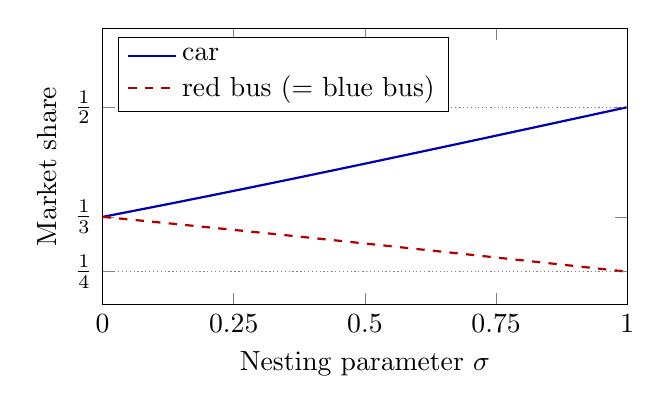
\begin{tikzpicture}
\begin{axis}[width=0.68\textwidth, height=0.42\textwidth,
  xlabel={Nesting parameter $\sigma$}, ylabel={Market share},
  xmin=0, xmax=1, ymin=0.2, ymax=0.62,
  ytick={0.25,0.3333,0.5}, yticklabels={$\frac{1}{4}$,$\frac{1}{3}$,$\frac{1}{2}$},
  xtick={0,0.25,0.5,0.75,1},
  domain=0:0.999, samples=120, legend style={at={(0.03,0.97)}, anchor=north west}, legend cell align=left,
  every axis plot/.append style={thick}]
\addplot[blue!70!black] {1/(1+2^(1-x))};
\addlegendentry{car}
\addplot[red!70!black, dashed] {2^(-x)/(1+2^(1-x))};
\addlegendentry{red bus (= blue bus)}
\addplot[gray, thin, densely dotted, domain=0:1] {0.5};
\addplot[gray, thin, densely dotted, domain=0:1] {0.25};
\end{axis}
\end{tikzpicture}
\caption{Red bus, blue bus. Shares of the car and of each bus from \eqref{eq:07-redbus} when the two buses form one
nest and the car is alone in its nest, all with equal mean utilities. The logit ($\sigma = 0$) gives
$\frac{1}{3}$ to each mode. As $\sigma \to 1$ the car keeps $\frac{1}{2}$ and the buses split the other half.}
\label{fig:07-redbus}
\end{figure}

\subsection{Estimation}\label{sec:07-nl-estimation}

Like the logit, the nested logit can be inverted in closed form, and the inverted equation is linear in the
parameters.

\begin{proposition}[Nested logit inversion]\label{prop:07-nl-inversion}
Under \cref{asm:07-nl}, let the observed shares $s_j > 0$ and $s_0 > 0$ sum to one. Let
$\bar s_g = \sum_{k\in g}s_k$ be the observed nest shares and $s_{j \mid g} = \frac{s_j}{\bar s_g}$ the observed
within-nest shares. For a given $\sigma \in [0, 1)$, the unique mean utilities that reproduce the observed shares
are
\begin{equation}\label{eq:07-nl-delta}
\delta_j = \ln s_j - \ln s_0 - \sigma\ln s_{j \mid g} .
\end{equation}
With $\delta_{jt} = x_{jt}\beta - \alpha p_{jt} + \xi_{jt}$ in market $t$, the shares satisfy
\begin{equation}\label{eq:07-nl-regression}
\ln s_{jt} - \ln s_{0t} = x_{jt}\beta - \alpha p_{jt} + \sigma\ln s_{j \mid g, t} + \xi_{jt} .
\end{equation}
\end{proposition}

\begin{proof}
Start from the expression for $\ln s_j$ derived before \eqref{eq:07-nl-dlns} and subtract
$\ln s_0 = -\ln(1 + \sum_h D_h^{1-\sigma})$:
\begin{equation*}
\ln s_j - \ln s_0 = \frac{\delta_j}{1-\sigma} - \sigma\ln D_g .
\end{equation*}
This still contains the unobserved inclusive sum. The within-nest share gives
$\ln s_{j \mid g} = \frac{\delta_j}{1-\sigma} - \ln D_g$, so
$\ln D_g = \frac{\delta_j}{1-\sigma} - \ln s_{j \mid g}$. Substituting,
\begin{align*}
\ln s_j - \ln s_0 &= \frac{\delta_j}{1-\sigma} - \frac{\sigma\delta_j}{1-\sigma} + \sigma\ln s_{j \mid g} \\
&= \delta_j + \sigma\ln s_{j \mid g} ,
\end{align*}
which rearranges to \eqref{eq:07-nl-delta}. Any $\delta$ that reproduces the shares must therefore equal
\eqref{eq:07-nl-delta}.

To show that \eqref{eq:07-nl-delta} reproduces the shares, compute its inclusive sums. Using
$s_k = \bar s_g s_{k \mid g}$,
\begin{equation*}
e^{\frac{\delta_k}{1-\sigma}} = \Big(\frac{s_k}{s_0}\Big)^{\frac{1}{1-\sigma}}s_{k \mid g}^{-\frac{\sigma}{1-\sigma}}
= \Big(\frac{\bar s_g}{s_0}\Big)^{\frac{1}{1-\sigma}}s_{k \mid g} .
\end{equation*}
Summing over $k \in g$ gives $D_g = \big(\frac{\bar s_g}{s_0}\big)^{\frac{1}{1-\sigma}}$, so
$D_g^{1-\sigma} = \frac{\bar s_g}{s_0}$. The model's within-nest share is then
$\frac{e^{\frac{\delta_j}{1-\sigma}}}{D_g} = s_{j \mid g}$. Its nest share is
$\frac{\bar s_g s_0^{-1}}{1 + \sum_h \bar s_h s_0^{-1}} = \frac{\bar s_g}{s_0 + \sum_h \bar s_h} = \bar s_g$, because the
shares sum to one. Both factors match the data, so the model reproduces every $s_j$.
\end{proof}

\citet[eqs.~26--28, p.~253]{Berry1994} reaches the same equation by eliminating $D_g$ through the nest share,
$D_g^{1-\sigma} = \frac{\bar s_g}{s_0}$, the identity used in the second half of the proof
(\cref{sec:07-berry-examples} follows his route). The regression \eqref{eq:07-nl-regression} is the logit
regression \eqref{eq:07-logit-inversion} with one additional regressor, the log within-nest share. Its coefficient is the nesting parameter. \citet[n.~7]{Berry1994} notes that
the formula extends, ``easily (but somewhat tediously)'', to several levels of nests and to nest-specific
parameters $\sigma_g$. \Cref{sec:07-nl-twolevel} carries out the two-level case.

\casehead{One inside nest}
The cheapest nesting puts all inside goods in one nest and the outside good in the other. Then
$s_{j \mid g} = \frac{s_j}{1 - s_0}$, and \eqref{eq:07-nl-regression} becomes
\begin{equation}\label{eq:07-nl-onenest}
\ln s_{jt} - \ln s_{0t} = x_{jt}\beta - \alpha p_{jt} + \sigma\ln\frac{s_{jt}}{1 - s_{0t}} + \xi_{jt} .
\end{equation}
The model requires no classification of products, so it is often run as a robustness check on the logit. With one
inside nest and inclusive sum $D$, the share formula is
\begin{equation*}
s_j = \frac{e^{\frac{\delta_j}{1-\sigma}}D^{-\sigma}}{1 + D^{1-\sigma}} = \frac{e^{\frac{\delta_j}{1-\sigma}}}{D^{\sigma} + D} ,
\end{equation*}
which is the form \citet[eq.~3]{Einav2007} uses for movies (\cref{sec:07-einav}).

The nesting parameter then measures how much additional products expand the category rather than steal
business from rivals. Suppose the market has $J$ identical inside products with mean utility $\delta$. The total
inside share is $1 - s_0 = \frac{J^{1-\sigma}e^{\delta}}{1 + J^{1-\sigma}e^{\delta}}$, whose elasticity with respect to $J$
is $(1-\sigma)s_0$. At $\sigma = 0$ each new product draws consumers from the outside good as in the logit. As
$\sigma \to 1$ new copies only divide a fixed category. Raising the mean utility $\delta_j$ of an existing product is different. At given shares,
$\frac{\partial\ln(1 - s_0)}{\partial\delta_j} = s_0 s_{j \mid g}$ for every $\sigma$, which is the logit value
$\frac{s_0 s_j}{1 - s_0}$. A uniform rise $\Delta$ in all inside prices multiplies
$D^{1-\sigma}$ by $e^{-\alpha\Delta}$, so
\begin{equation*}
\frac{\dd\ln(1 - s_0)}{\dd\Delta} = -\alpha s_0 ,
\end{equation*}
the same as in the logit. For a given price coefficient, $\sigma$ leaves the category response unchanged. It raises
the own elasticity of a product with a small within-nest share by a factor close to $\frac{1}{1-\sigma}$.
\Citet[p.~1774]{MillerWeinberg2017} use the one-nest model for beer. Their richer specifications add random
coefficients that interact consumer income with price and product characteristics (Table~IV). They note that the nesting parameter keeps the elasticities from being overly sensitive to the
assumed market size (\cref{sec:07-market-size,ch:mergers}).

\casehead{Endogeneity of the within-nest share}
The within-nest share depends on $\xi_{jt}$. From \eqref{eq:07-nl-share},
$\frac{\partial\ln s_{j \mid g}}{\partial\xi_j} = \frac{1 - s_{j \mid g}}{1-\sigma} > 0$, so the regressor
$\ln s_{j \mid g, t}$ is positively correlated with the error. A high-quality product also lowers the within-nest
shares of its nest-mates, so the regressor is endogenous for every product in the nest. OLS therefore tends to
bias $\hat\sigma$ upward, toward one. Prices are endogenous as in the logit (\cref{sec:07-endogeneity}). Estimating
\eqref{eq:07-nl-regression} needs at least two excluded instruments, one for $p_{jt}$ and one for
$\ln s_{j \mid g, t}$, and the two must move the regressors in different ways.

Instruments for the within-nest share shift the crowding of a product's nest without shifting its own unobserved
quality. Common choices follow.
\begin{itemize}
  \item The number of products in the nest, $J_{gt}$. More nest-mates lower $s_{j \mid g}$ mechanically.
  \item Sums or averages of the characteristics of the other products in the nest. \citet[p.~254]{Berry1994}
  suggests ``the characteristics of other firms in the group''. These are the nest-level versions of the BLP
  instruments of \cref{sec:07-instruments}, and the differentiation instruments of \citet{GandhiHoude2019}
  refine them.
  \item Cost shifters of the other products in the nest, which move their prices and hence $s_{j \mid g}$.
  \item Application-specific counts. \citet{Einav2007} uses the number of movies showing in the same week.
\end{itemize}
These instruments are valid if the number and characteristics of nest-mates are mean independent of $\xi_{jt}$.
Endogenous entry threatens this condition. Firms add products to nests and markets where demand is high, so
$J_{gt}$ may be correlated with $\xi_{jt}$. Product and market fixed effects absorb persistent demand differences
and reduce the concern, provided entry does not respond to transitory shocks.

\casehead{What identifies $\sigma$}
Fix a product's mean utility and add a rival to its nest. The rival lowers $\ln s_{j \mid g}$. By
\eqref{eq:07-nl-regression}, it lowers $\ln\frac{s_j}{s_0}$ by $\sigma$ times as much. A rival added to a different
nest changes neither the within share nor the ratio $\frac{s_j}{s_0}$. With $\sigma = 0$ the ratio $\frac{s_j}{s_0}$ does not respond at all, which is IIA. With
$\sigma$ near one it falls almost one for one with the within share. A rival that does not beat the best product in
the nest then steals customers almost only from its nest-mates. A better rival also draws from the outside good,
because it raises the nest's best mean utility. Comparing the same product across markets with exogenously different nest-mates therefore traces out
$\sigma$. On the supply side, \citet[pp.~255--256]{Berry1994} adds that the joint behavior of prices, product shares
and group shares in the pricing equation helps identify $\sigma$ (\cref{sec:07-nl-pricing}). Estimates of
$\sigma$ outside $[0, 1)$ signal a misspecified tree or invalid instruments (\cref{lem:07-nl-gev}).

\casehead{Estimation from individual choices}
With data on individual choices, the nested logit can be estimated by maximum likelihood, as the logit is in
\cref{sec:07-micro-ml}. Let consumer $i$ have utility index $V_{ij}$ in place of $\delta_j$, with the outside good
normalized to zero. For $j$ in nest $g$, split the index into a part $z_{ig}\gamma$ that is constant within the nest
and a part $w_{ij}b$ that varies within it, $V_{ij} = z_{ig}\gamma + w_{ij}b$. The inclusive sum
$D_{ig} = \sum_{k \in g}e^{\frac{V_{ik}}{1-\sigma}}$ then satisfies
\begin{equation*}
\ln D_{ig} = \frac{z_{ig}\gamma}{1-\sigma} + I_{ig}, \qquad
I_{ig} = \ln\sum_{k \in g}\exp\Big(\frac{w_{ik}b}{1-\sigma}\Big) .
\end{equation*}
Substituting into \cref{prop:07-nl-shares}, the choice probability factors into a within-nest and a nest
probability,
\begin{equation}\label{eq:07-nl-sequential}
P_{ij \mid g} = \exp\Big(\frac{w_{ij}b}{1-\sigma} - I_{ig}\Big), \qquad
P_{ig} = \frac{\exp\big(z_{ig}\gamma + (1-\sigma)I_{ig}\big)}{1 + \sum_h\exp\big(z_{ih}\gamma + (1-\sigma)I_{ih}\big)} .
\end{equation}
The log-likelihood sums $\ln P_{ij \mid g} + \ln P_{ig}$ over the observed choices. Unlike the logit likelihood of
\cref{prop:07-ml-concave}, it ``is not concave in all parameters, and is highly non-linear in the inclusive value
coefficients'' \citep[p.~1426]{McFadden1984}. A search can then stop at a local maximum, so it should start from
several points.

\Cref{eq:07-nl-sequential} suggests a \emph{sequential estimator}. The first step fits a logit to the choices within
each nest, which estimates $\frac{b}{1-\sigma}$. The second step computes the estimated inclusive values $\hat I_{ig}$
and fits a logit to the choice of nest, with regressors $z_{ig}$ and $\hat I_{ig}$. The coefficient on $\hat I_{ig}$
estimates $1 - \sigma$. Each step is a concave logit problem. McFadden notes that the estimator is consistent but
often inefficient. Its second-step standard errors are wrong, because the inclusive values are estimated, and
correction formulae exist (p.~1426). One Newton step on the full likelihood from the sequential estimates is
asymptotically equivalent to full maximum likelihood. In practice the strong nonlinearity can make this one-step
estimator erratic, so several iterations may be needed. In McFadden's housing example (\cref{tab:07-mcfadden-housing})
only \textit{OPCOST} and \textit{YNH} vary among renters, so only their coefficients enter the first step. There the
two estimators agree to the third decimal place, with log-likelihoods of $-10.7868$ for the sequential estimates and
$-10.7862$ at the full maximum (p.~1432).

\casehead{Choosing the nests}
The nests must be fixed before estimation, a limitation the nested logit shares with multi-stage budgeting
(\cref{ch:aids}). The classification is often unclear. Is a minivan a car or a truck? Are store-brand and
national-brand cereals in the same nest? Is a family sedan closer to a compact car or to a luxury car? Different
nestings imply different substitution patterns, and the data may not discriminate between them. With several
levels the order of the nests also matters. \citet[n.~18]{Nevo2000a} notes that classifying computers first into
branded and unbranded and then into frontier and non-frontier technology implies different substitution than the
reverse order, even with the same classification. Practical checks include estimating nest-specific parameters
$\sigma_g$, comparing non-nested trees by fit, and checking that all estimates lie in $[0, 1)$.

\casehead{A Monte Carlo experiment}
We illustrate these points with a simulation. Each sample has $500$ markets with two inside nests and an outside
good. In the main design the number of products in each nest is drawn uniformly from $\{1, \dots, 5\}$ in every
market. Each product has its own owner. Mean utility is $\delta_j = \beta_0 + \beta_xx_j - \alpha p_j + \xi_j$ with
$\beta_0 = 2$, $\beta_x = 1$, $\alpha = 1$ and $\sigma = 0.5$. Marginal cost is
$c_j = \exp(0.5 + 0.25x_j + 0.25w_j + 0.1\xi_j + 0.25\omega_j)$, where $x_j$, $\xi_j$, $w_j$ and $\omega_j$
are independent standard normal variables. Prices are the single-product Bertrand-Nash equilibrium of
\cref{prop:07-nl-markup}. The average outside share is $0.28$ and the average within-nest share is $0.33$. There
are five excluded instruments. The first two are the own cost shifter $w_j$ and the number of products in the own
nest. The other three are sums over rival products. They add up $x$ over the other products in the own nest, $x$
over the products of the other nest, and $w$ over the other products in the own nest. We draw $500$ samples. A second design fixes three products in every nest, so the count
instrument disappears.

\begin{table}[htbp]
\centering
\caption{Monte Carlo estimates of the nested logit regression}\label{tab:07-mc-nl}
\small
\begin{tabular}{@{}lcccccc@{}}
\toprule
 & & \multicolumn{4}{c}{Nest sizes vary across markets} & Fixed size \\
\cmidrule(lr){3-6}\cmidrule(lr){7-7}
Parameter & True & OLS & IV, price only & IV, both & Logit IV & IV, both \\
\midrule
$\beta_0$ & 2.0 & 0.920 & 2.258 & 2.003 & 1.561 & 1.997 \\
 & & (0.055) & (0.120) & (0.115) & (0.204) & (0.121) \\
$\beta_x$ & 1.0 & 0.462 & 0.760 & 1.001 & 1.417 & 0.998 \\
 & & (0.022) & (0.036) & (0.034) & (0.053) & (0.047) \\
$\alpha$ & 1.0 & 0.334 & 0.870 & 1.002 & 1.228 & 0.998 \\
 & & (0.022) & (0.049) & (0.045) & (0.082) & (0.057) \\
$\sigma$ & 0.5 & 0.801 & 0.787 & 0.499 & 0 & 0.500 \\
 & & (0.009) & (0.010) & (0.019) &  & (0.031) \\
\addlinespace
Mean own elasticity & 3.83 & 2.91 & 7.16 & 3.83 & 2.71 & 3.83 \\
 & & (0.19) & (0.40) & (0.19) & (0.18) & (0.20) \\
\bottomrule
\end{tabular}
\par\smallskip
\begin{minipage}{0.95\textwidth}
\footnotesize Notes: Means across 500 simulated samples of 500 markets, with standard deviations across samples
in parentheses. Columns 3 to 6 use the main design, in which each of the two nests has between one and five
products. Column 7 fixes three products per nest. ``IV, price only'' instruments the price and treats
$\ln s_{j \mid g}$ as exogenous. ``IV, both'' instruments both. ``Logit IV'' imposes $\sigma = 0$. The mean own
elasticity averages $\varepsilon_j$ from \eqref{eq:07-nl-elast} over products at the estimated parameters. Its
true value is $3.83$ in the main design and $3.82$ in the fixed-size design. Mean first-stage $F$ statistics of
the excluded instruments are $304$ for price and $277$ for $\ln s_{j \mid g}$ in the main design, and $336$ and
$183$ in the fixed-size design. Computed by \texttt{figures/ch07/src/mc\_nested\_logit.py}.
\end{minipage}
\end{table}

\Cref{tab:07-mc-nl} reports the results. OLS gives $\hat\sigma = 0.801$ against a true value of $0.5$ and cuts
the price coefficient to a third of its true value. Instrumenting the price alone fixes most of the price bias,
with $\hat\alpha = 0.870$. The nesting parameter stays near $0.79$, however, and the implied own elasticity of
$7.16$ is almost twice the true value of $3.83$. Treating the within-nest share as exogenous is therefore costly
even with a valid price instrument. Instrumenting both regressors recovers every parameter. Imposing the logit
($\sigma = 0$) with the same instruments biases $\hat\alpha$ and $\hat\beta_x$ upward. It also understates the mean
own elasticity by about 29 percent, because the factor $\frac{1}{1-\sigma}$ is missing from the elasticity formula.
With fixed nest sizes, the characteristics of nest-mates still identify $\sigma$. The standard deviation of
$\hat\sigma$ rises from $0.019$ to $0.031$, which shows that variation in the number of products adds
information.

\subsection{Pricing with nested logit demand}\label{sec:07-nl-pricing}

The nested logit keeps the analytic markups of the logit. We first treat single-product firms and then derive a
closed form for multi-product firms.

\begin{proposition}[Single-product markups]\label{prop:07-nl-markup}
Under \cref{asm:07-nl} with constant marginal cost $mc_j$, the first-order condition of a single-product firm
selling $j \in g$ implies
\begin{equation}\label{eq:07-nl-markup}
p_j - mc_j = \frac{1-\sigma}{\alpha\big[1 - \sigma s_{j \mid g} - (1-\sigma)s_j\big]} .
\end{equation}
\end{proposition}

\begin{proof}
The firm maximizes $M(p_j - mc_j)s_j(p)$. The first-order condition is
$s_j + (p_j - mc_j)\frac{\partial s_j}{\partial p_j} = 0$. By \eqref{eq:07-nl-own},
\begin{equation*}
\frac{\partial s_j}{\partial p_j} = -\frac{\alpha s_j}{1-\sigma}\big[1 - \sigma s_{j \mid g} - (1-\sigma)s_j\big] .
\end{equation*}
Substituting and dividing by $s_j > 0$,
\begin{equation*}
1 - \frac{\alpha(p_j - mc_j)}{1-\sigma}\big[1 - \sigma s_{j \mid g} - (1-\sigma)s_j\big] = 0 ,
\end{equation*}
which rearranges to \eqref{eq:07-nl-markup}.
\end{proof}

This is equation (33) of \citet[p.~255]{Berry1994}. With $mc_j = w_j\gamma + \omega_j$ it becomes a linear supply
equation, $p_j = w_j\gamma + \frac{1-\sigma}{\alpha[1 - \sigma s_{j \mid g} - (1-\sigma)s_j]} + \omega_j$, which can be
estimated jointly with \eqref{eq:07-nl-regression} as in \cref{sec:07-cost-recovery}. When $\sigma = 0$ only the
product share matters, as in the logit markup $\frac{1}{\alpha(1-s_j)}$. As $\sigma \to 1$ with $s_{j \mid g} < 1$
held fixed, only the within-nest share matters. A product alone in its nest keeps the logit markup for every
$\sigma$. The markup is at least $\frac{1-\sigma}{\alpha}$, so the logit floor $\frac{1}{\alpha}$ falls as products become
closer substitutes. If $\sigma \to 1$ and a nest holds many products with small within shares, the markup goes to
zero, which is Bertrand competition with perfect substitutes.

\begin{proposition}[Multi-product markups]\label{prop:07-nl-multi}
Under \cref{asm:07-nl} with constant marginal costs, let firm $f$ own the products $\mathcal{J}_f$. Write
$S_{fh} = \sum_{k \in \mathcal{J}_f \cap h}s_k$ for its combined share in nest $h$ and
$S_{f \mid h} = \frac{S_{fh}}{s_h}$ for its share within nest $h$. At an interior Bertrand-Nash equilibrium, all of
the firm's products in a nest $g$ carry the same markup,
\begin{equation}\label{eq:07-nl-multi}
m_{fg} = \frac{1-\sigma}{\alpha\big(1 - \sigma S_{f \mid g}\big)\big(1 - \Phi_f\big)}, \qquad
\Phi_f = \sum_{h} \frac{(1-\sigma)S_{fh}}{1 - \sigma S_{f \mid h}} ,
\end{equation}
where the sum runs over the nests in which $f$ sells, and $0 \le \Phi_f < 1$.
\end{proposition}

\begin{proof}
Write $m_k = p_k - mc_k$. The firm maximizes $M\sum_{k\in\mathcal{J}_f}m_ks_k(p)$. The first-order condition for
$j \in \mathcal{J}_f \cap g$ is
\begin{equation*}
s_j + \sum_{k \in \mathcal{J}_f}m_k\frac{\partial s_k}{\partial p_j} = 0 .
\end{equation*}
By \eqref{eq:07-nl-dlns} with the roles of $j$ and $k$ exchanged, and $\frac{\partial\delta_j}{\partial p_j} = -\alpha$,
\begin{equation*}
\frac{\partial s_k}{\partial p_j} = -\alpha s_k\Big[\frac{\indic\{k = j\}}{1-\sigma} - \frac{\sigma}{1-\sigma}s_{j \mid g}\indic\{k \in g\} - s_j\Big] .
\end{equation*}
Substituting into the first-order condition,
\begin{equation*}
s_j - \frac{\alpha m_js_j}{1-\sigma} + \frac{\alpha\sigma}{1-\sigma}s_{j \mid g}\sum_{k\in\mathcal{J}_f\cap g}m_ks_k
+ \alpha s_j\sum_{k\in\mathcal{J}_f}m_ks_k = 0 .
\end{equation*}
Divide by $s_j$ and use $\frac{s_{j \mid g}}{s_j} = \frac{1}{s_g}$ and $\frac{s_k}{s_g} = s_{k \mid g}$. Multiplying by
$\frac{1-\sigma}{\alpha}$,
\begin{equation*}
m_j = \frac{1-\sigma}{\alpha} + \sigma\sum_{k\in\mathcal{J}_f\cap g}m_ks_{k \mid g} + (1-\sigma)\sum_{k\in\mathcal{J}_f}m_ks_k .
\end{equation*}
The right side depends on $j$ only through its nest $g$. Hence $m_j = m_{fg}$ for every
$j \in \mathcal{J}_f \cap g$. The first sum then equals $m_{fg}S_{f \mid g}$ and the second equals
$\sum_h m_{fh}S_{fh}$. Let $A_f = \frac{1-\sigma}{\alpha} + (1-\sigma)\sum_h m_{fh}S_{fh}$, which does not depend on
$g$. Then
\begin{equation*}
m_{fg}\big(1 - \sigma S_{f \mid g}\big) = A_f, \qquad\text{so}\qquad m_{fg} = \frac{A_f}{1 - \sigma S_{f \mid g}} .
\end{equation*}
Substituting back into the definition of $A_f$,
\begin{equation*}
A_f = \frac{1-\sigma}{\alpha} + A_f\sum_h\frac{(1-\sigma)S_{fh}}{1 - \sigma S_{f \mid h}} = \frac{1-\sigma}{\alpha} + A_f\Phi_f ,
\end{equation*}
so $A_f = \frac{1-\sigma}{\alpha(1 - \Phi_f)}$, which gives \eqref{eq:07-nl-multi}. For the bound, each term of
$\Phi_f$ equals $s_h\frac{(1-\sigma)S_{f \mid h}}{1 - \sigma S_{f \mid h}} \le s_h$, since $(1-\sigma)x \le 1 - \sigma x$ for
$x \le 1$. Hence $\Phi_f \le \sum_h s_h \le 1 - s_0 < 1$.
\end{proof}

Two checks confirm the formula. For a single product, $S_{f \mid g} = s_{j \mid g}$, $S_{fg} = s_j$ and
$\Phi_f = \frac{(1-\sigma)s_j}{1 - \sigma s_{j \mid g}}$. The product
$(1 - \sigma s_{j \mid g})(1 - \Phi_f)$ equals $1 - \sigma s_{j \mid g} - (1-\sigma)s_j$, which gives
\eqref{eq:07-nl-markup}. At $\sigma = 0$, $\Phi_f = \sum_h S_{fh} = S_f$ and $m_{fg} = \frac{1}{\alpha(1 - S_f)}$, the
logit result of \cref{prop:07-logit-multi}. The formula has two layers of internalized cannibalization. The
factor $1 - \sigma S_{f \mid g}$ captures recapture within the nest, which grows with $\sigma$ and with the firm's
within-nest share. The factor $1 - \Phi_f$ captures recapture across all of the firm's nests through the common
outside option.

\begin{example}[Ownership and markups]\label{ex:07-nl-markups}
Consider a market with two inside nests. Nest A has three products with shares $0.15$ each, nest B has two products
with shares $0.10$ each, and $s_0 = 0.35$. Let $\alpha = 1$. We compute the markup of a nest-A product implied by
\eqref{eq:07-nl-multi} at these observed shares, as one does when recovering costs from data.
\Cref{tab:07-nl-markup-example} reports three ownership structures. Under the logit, joint ownership of two nest-A
products raises the markup by 21.4 percent, and joint ownership of a nest-A and a nest-B product raises it by
13.3 percent. At $\sigma = 0.5$ the same changes raise it by 46.8 and 7.9 percent. At $\sigma = 0.8$ they raise it
by 73.0 and 3.6 percent. Common ownership matters far more within a nest than across nests once $\sigma$ is large.
The logit cannot make this distinction, which is why merger simulation with logit demand spreads price effects
evenly (\cref{ch:mergers}).
\end{example}

\begin{table}[htbp]
\centering
\caption{Implied markups of a nest-A product under alternative ownership}\label{tab:07-nl-markup-example}
\small
\begin{tabular}{@{}lccc@{}}
\toprule
Ownership & $\sigma = 0$ & $\sigma = 0.5$ & $\sigma = 0.8$ \\
\midrule
Single-product firms & 1.176 & 0.659 & 0.284 \\
One firm owns two nest-A products & 1.429 & 0.968 & 0.492 \\
One firm owns a nest-A and a nest-B product & 1.333 & 0.711 & 0.295 \\
\addlinespace
Percent increase, two nest-A products & 21.4 & 46.8 & 73.0 \\
Percent increase, nest-A and nest-B products & 13.3 & 7.9 & 3.6 \\
\bottomrule
\end{tabular}
\par\smallskip
\begin{minipage}{0.8\textwidth}
\footnotesize Notes: Illustrative shares $0.15$ for each of three nest-A products, $0.10$ for each of two nest-B
products, $s_0 = 0.35$, and $\alpha = 1$. Markups in dollars from \eqref{eq:07-nl-multi} at fixed shares. Computed by
\texttt{figures/ch07/src/nl\_markup\_example.py}.
\end{minipage}
\end{table}

The equilibrium can be computed in several ways. Iterating on the markup equation,
$p \leftarrow mc + m(p)$, is the simplest method. In our Monte Carlo experiment it settled into a two-cycle in some
markets with one dominant product. Iterating on exact best responses converged in every market of the experiment.
Each best response solves a one-dimensional equation, because the left side of the first-order condition
\eqref{eq:07-nl-markup} rises in the own price and the right side falls.

\subsection{The two-level nested logit}\label{sec:07-nl-twolevel}

Some markets have two natural dimensions of grouping. Cars differ by segment and by country of origin. Painkillers
differ by active substance and by form. The two-level nested logit, as used by \citet{Verboven1996}, splits each group $g$
into subgroups $h$ and adds a second nest taste. For product $j$ in subgroup $h$ of group $g$,
\begin{equation}\label{eq:07-nl2-utility}
u_{ij} = \delta_j + \zeta_{ig} + (1 - \sigma_2)\zeta_{ihg} + (1 - \sigma_1)\epsilon_{ij} ,
\end{equation}
with the outside good alone in its group. The parameter $\sigma_1$ measures the correlation of utilities within a
subgroup and $\sigma_2$ the correlation within a group.

The model is consistent with utility maximization when $0 \le \sigma_2 \le \sigma_1 < 1$. To see why, apply
\cref{lem:07-cardell} twice. Write the subgroup part of \eqref{eq:07-nl2-utility} as
\begin{equation*}
(1-\sigma_2)\Big[\zeta_{ihg} + \frac{1-\sigma_1}{1-\sigma_2}\epsilon_{ij}\Big] .
\end{equation*}
The bracket is Gumbel if $\zeta_{ihg} \sim C(\tau)$ with $1 - \tau = \frac{1-\sigma_1}{1-\sigma_2}$, which requires
$\tau \in [0, 1)$, that is $\sigma_1 \ge \sigma_2$. The group part, $\zeta_{ig}$ plus $1 - \sigma_2$
times a Gumbel variable, is then Gumbel if $\zeta_{ig} \sim C(\sigma_2)$.

The shares follow from the sequential derivation in the proof of \cref{prop:07-nl-shares}, applied level by level.
Within subgroup $hg$ the terms $\zeta_{ig}$ and $\zeta_{ihg}$ are common to all products, so the choice of product is
a logit with scale $1 - \sigma_1$. Let $D_{hg} = \sum_{k \in hg}e^{\frac{\delta_k}{1-\sigma_1}}$. By max-stability of
the Gumbel, the best utility in subgroup $hg$ is
\begin{equation*}
(1-\sigma_1)\ln D_{hg} + \zeta_{ig} + (1-\sigma_2)\Big[\zeta_{ihg} + \frac{1-\sigma_1}{1-\sigma_2}\tilde\epsilon_{ihg}\Big],
\end{equation*}
where $\tilde\epsilon_{ihg}$ is standard Gumbel. The bracket is standard Gumbel, as shown above, and $\zeta_{ig}$ is
common to all subgroups of $g$. So the choice of subgroup within $g$ is a logit with scale $1 - \sigma_2$ in the
values $(1-\sigma_1)\ln D_{hg}$, which gives $s_{h \mid g}$ below. Let $D_g = \sum_{h \in g}D_{hg}^{\frac{1-\sigma_1}{1-\sigma_2}}$.
Applying max-stability once more, the best utility in group $g$ is $(1-\sigma_2)\ln D_g + \zeta_{ig} +
(1-\sigma_2)\tilde\epsilon_{ig}$ with $\tilde\epsilon_{ig}$ standard Gumbel. Since $\zeta_{ig} \sim C(\sigma_2)$, the
last two terms form a standard Gumbel variable. The choice of group is therefore a logit in the values
$(1-\sigma_2)\ln D_g$, with $0$ for the outside good. Together these steps give
\begin{equation}\label{eq:07-nl2-shares}
s_{j \mid hg} = \frac{e^{\frac{\delta_j}{1-\sigma_1}}}{D_{hg}}, \qquad
s_{h \mid g} = \frac{D_{hg}^{\frac{1-\sigma_1}{1-\sigma_2}}}{D_g}, \qquad
s_g = \frac{D_g^{1-\sigma_2}}{1 + \sum_{g'}D_{g'}^{1-\sigma_2}} ,
\end{equation}
with the inclusive sums $D_{hg}$ and $D_g$ defined above. The product share is
$s_j = s_{j \mid hg}\,s_{h \mid g}\,s_g$.

\casehead{The estimating equation}
Taking logs of the three factors and subtracting $\ln s_0 = -\ln(1 + \sum_{g'}D_{g'}^{1-\sigma_2})$,
\begin{align*}
\ln s_j - \ln s_0 &= \frac{\delta_j}{1-\sigma_1} - \ln D_{hg} + \frac{1-\sigma_1}{1-\sigma_2}\ln D_{hg} - \ln D_g + (1-\sigma_2)\ln D_g \\
&= \frac{\delta_j}{1-\sigma_1} - \frac{\sigma_1 - \sigma_2}{1-\sigma_2}\ln D_{hg} - \sigma_2\ln D_g .
\end{align*}
Eliminate the group inclusive sum first. From the subgroup share,
$\ln D_g = \frac{1-\sigma_1}{1-\sigma_2}\ln D_{hg} - \ln s_{h \mid g}$. Substituting,
\begin{align*}
\ln s_j - \ln s_0 &= \frac{\delta_j}{1-\sigma_1} - \Big[\frac{\sigma_1 - \sigma_2}{1-\sigma_2} + \frac{\sigma_2(1-\sigma_1)}{1-\sigma_2}\Big]\ln D_{hg} + \sigma_2\ln s_{h \mid g} \\
&= \frac{\delta_j}{1-\sigma_1} - \sigma_1\ln D_{hg} + \sigma_2\ln s_{h \mid g} ,
\end{align*}
because $\sigma_1 - \sigma_2 + \sigma_2 - \sigma_1\sigma_2 = \sigma_1(1-\sigma_2)$. Next eliminate the subgroup inclusive
sum using $\ln D_{hg} = \frac{\delta_j}{1-\sigma_1} - \ln s_{j \mid hg}$:
\begin{equation}\label{eq:07-nl2-regression}
\ln s_{jt} - \ln s_{0t} = x_{jt}\beta - \alpha p_{jt} + \sigma_1\ln s_{j \mid hg, t} + \sigma_2\ln s_{h \mid g, t} + \xi_{jt} .
\end{equation}
The regression adds the log within-subgroup share and the log subgroup share within the group. When
$\sigma_1 = \sigma_2 = \sigma$ the two terms combine into $\sigma\ln s_{j \mid g}$, the one-level model with groups as
nests. Both shares are endogenous, so the equation needs three excluded instruments, for example counts and
characteristics of products in the same subgroup and in the same group.

\casehead{Substitution}
Differentiating the logs of \eqref{eq:07-nl2-shares} as in \cref{sec:07-nl-substitution} gives, for $j$ in
subgroup $h$ of group $g$,
\begin{equation*}
\frac{\partial\ln s_j}{\partial\delta_k} = \frac{\indic\{j = k\}}{1-\sigma_1}
- \Big(\frac{1}{1-\sigma_1} - \frac{1}{1-\sigma_2}\Big)s_{k \mid hg}\indic\{k \in hg\}
- \frac{\sigma_2}{1-\sigma_2}s_{k \mid g}\indic\{k \in g\} - s_k ,
\end{equation*}
where $s_{k \mid g} = s_{k \mid hg}s_{h \mid g}$ is $k$'s share within the group. Cross elasticities are largest within
a subgroup, intermediate within a group, and smallest across groups when $\sigma_1 \ge \sigma_2 \ge 0$.

\casehead{Applications}
\citet{Goldberg1995} uses a multi-level nested logit for cars (\cref{ch:blp}).
\citet{Verboven1996} applies the two-level model to price discrimination in the European car market. The groups are
six classes (mini and small, medium, large, executive, luxury and sports). Each class splits into domestic and
foreign cars \citep[pp.~251 and 254]{Verboven1996}.
\citet{BjornerstedtVerboven2016} nest analgesics by active substance and by form. They compare merger predictions with
the outcome of an actual merger (\cref{ch:mergers}). Their study is one of the ex-post evaluations of merger
simulation listed by \citet[p.~231]{AskerNocke2021}. \citet{BerryCarnallSpiller2006} combine a nested logit with two
consumer types for airline travel and write the nesting parameter as $\lambda = 1 - \sigma$ (\cref{ch:airlines}).
\citet{MillerWeinberg2017} add random coefficients to the one-nest model (\cref{ch:mergers}).

\subsection{Other GEV models and the limits of nesting}\label{sec:07-gev-other}

Nested logit trees force a hierarchy. A product belongs to one nest at each level, and the order of the levels
matters. Other members of the GEV family relax these restrictions while keeping closed forms. A key property makes
them easy to build. A sum of GEV generating functions with nonnegative weights, at least one of them positive, is
again a GEV generating function, because (G1) to (G3) are preserved under such sums.

\citet{BresnahanSternTrajtenberg1997} propose the \emph{principles of differentiation GEV} model (PD GEV) for
personal computers. Each principle $d$ partitions the products into categories, for example branded versus
unbranded and frontier versus non-frontier technology. Every product belongs to one category under each principle.
A generating function of this kind is
\begin{equation}\label{eq:07-pdgev}
H(y) = y_0 + \sum_{d} a_d\sum_{c \in d}\Big(\sum_{j \in c}y_j^{\frac{1}{1-\sigma_d}}\Big)^{1-\sigma_d},
\qquad a_d \ge 0, \quad \sum_d a_d = 1 ,
\end{equation}
where $c$ runs over the categories of principle $d$ and $\sigma_d \in [0, 1)$. By \eqref{eq:07-gev-prob}, the share
of $j$ is a weighted average of nested logit expressions, one for each principle,
\begin{equation*}
s_j = \frac{\sum_d a_d\,D_{c_d(j)}^{1-\sigma_d}\,s_{j \mid c_d(j)}}{H(y)} .
\end{equation*}
Here $c_d(j)$ is $j$'s category under principle $d$. The terms $D_c$ and $s_{j \mid c}$ are the inclusive sum and the
within-category share, both computed with $\sigma_d$. Two products that share a category under either principle are closer
substitutes, and no principle has to come first. \citet[p.~525]{Nevo2000a} summarizes that the model removes the
ordering problem and otherwise ``retains all the advantages and disadvantages of the nested logit''.

The \emph{generalized nested logit} of \citet{WenKoppelman2001} lets a product belong to several nests with
allocation weights. This captures, for example, a minivan that is partly a car and partly a truck. The
\emph{ordered GEV} model of \citet[p.~409]{Small1987} applies to alternatives with a natural order.
Examples are the number of cars a household owns and the time of day of a work trip. Its taste shocks are correlated among alternatives
that are close in the order, and the correlation does not rise with their distance (pp.~409--410).

\casehead{What nesting does not fix}
Every GEV model keeps the closed forms because it keeps much of the logit's structure. Within a nest, substitution
remains proportional to shares, so differences between nest-mates are invisible to the model
\citep[p.~524]{Nevo2000a}. Own elasticities still rise almost in proportion to price
(\cref{sec:07-nl-substitution}). Tastes are not linked to consumer demographics, so the model cannot say who
substitutes to what. The nests are imposed before estimation. \citet[p.~230]{Hausman1997} concludes that the nested
logit ``can solve some of these problems but still suffers from the IIA problem at each level of choice''.
\citet[p.~916]{GrigolonVerboven2014} compare the nested logit and the random coefficients logit within a random
coefficients nested logit. They use a simulation study and data from the European car market. They reject both
special cases against the general model. The random coefficients logit gives different substitution patterns and a
wider market definition than the two nested models, but the predicted price effects of mergers are robust across
models.
Random coefficients, developed in \cref{ch:blp}, make substitution depend on continuous characteristics and on
demographics. \Cref{sec:07-limits} returns to this comparison with evidence.

\section{Welfare in logit models}\label{sec:07-welfare}

Discrete choice models measure consumer welfare in closed form. The GEV theorem gives the expected maximum utility,
and quasi-linear utility converts it into dollars. This section derives the log-sum formula for the logit and the
nested logit, applies it to price changes, product removal, product proliferation and new goods, and states its
limitations.

\subsection{The log-sum formula}\label{sec:07-logsum}

Let utility be quasi-linear in income $y_i$,
\begin{equation}\label{eq:07-ql-utility}
u_{ij} = \alpha(y_i - p_j) + x_j\beta + \xi_j + e_{ij}, \quad j \in \mathcal{J}, \qquad u_{i0} = \alpha y_i + e_{i0} ,
\end{equation}
where the shock vector $e_i$ has a GEV distribution with generating function $H$. In the logit $e_{ij}$ is the
Gumbel shock $\epsilon_{ij}$. In the nested logit it is the composite $\zeta_{ig} + (1-\sigma)\epsilon_{ij}$. Mean
utility relative to the outside good is $\delta_j = x_j\beta - \alpha p_j + \xi_j$ and $\delta_0 = 0$. The marginal
utility of income is $\alpha$ for every consumer. The \emph{expected consumer surplus} is the expected maximum utility
in dollars, defined up to an additive constant $C$ that cancels from every comparison.

\begin{proposition}[Log-sum consumer surplus]\label{prop:07-logsum}
Under \eqref{eq:07-ql-utility}, the expected compensating variation of a change from a choice set
$\mathcal{J}^0$ with mean utilities $\delta^0$ to a choice set $\mathcal{J}^1$ with mean utilities $\delta^1$ is
\begin{equation}\label{eq:07-dcs}
\Delta CS = \frac{1}{\alpha}\Big[\ln H\big(e^{\delta^1}\big) - \ln H\big(e^{\delta^0}\big)\Big].
\end{equation}
Here $H(e^{\delta}) = H(1, e^{\delta_1}, \dots, e^{\delta_J})$, and absent products have $e^{\delta_k} = 0$. Expected
consumer surplus per consumer is $CS = \frac{1}{\alpha}\ln H(e^{\delta}) + C$. In particular,
\begin{align}
\text{logit:}\qquad CS &= \frac{1}{\alpha}\ln\Big(1 + \sum_{k \in \mathcal{J}}e^{\delta_k}\Big) + C, \label{eq:07-cs-logit}\\
\text{nested logit:}\qquad CS &= \frac{1}{\alpha}\ln\Big(1 + \sum_{g=1}^G D_g^{1-\sigma}\Big) + C . \label{eq:07-cs-nl}
\end{align}
In both models $CS = -\frac{1}{\alpha}\ln s_0 + C$, and $\frac{\partial CS}{\partial p_j} = -s_j$.
\end{proposition}

\begin{proof}
Write $V_j = \alpha y + \delta_j$ for the deterministic utilities. With quasi-linear utility, the expected
compensating variation is the change in expected maximum utility divided by $\alpha$, as derived in
\eqref{eq:06-smallrosen}. Applying \cref{prop:07-gev}(iii) to the expected maximum before and after the change,
\begin{equation*}
\E[CV] = \frac{1}{\alpha}\Big[\ln H\big(e^{V^1}\big) - \ln H\big(e^{V^0}\big)\Big] .
\end{equation*}
Homogeneity (G1) gives $H(e^{V}) = H(e^{\alpha y}e^{\delta}) = e^{\alpha y}H(e^{\delta})$, so
$\ln H(e^V) = \alpha y + \ln H(e^{\delta})$. The income terms cancel, which proves \eqref{eq:07-dcs}. Equations
\eqref{eq:07-cs-logit} and \eqref{eq:07-cs-nl} substitute the two generating functions, with $y_0 = 1$.
In both functions the outside good enters linearly, so $H_0 = 1$ and \eqref{eq:07-gev-prob} gives
$s_0 = \frac{1}{H(e^{\delta})}$. Hence $\ln H(e^{\delta}) = -\ln s_0$. Finally, by \eqref{eq:07-gev-prob},
$\frac{\partial CS}{\partial p_j} = \frac{1}{\alpha}\cdot(-\alpha)\frac{\partial\ln H}{\partial\delta_j} = -s_j$.
\end{proof}

The formula is due to \citet{Williams1977}, \citet{SmallRosen1981} and \citet{McFadden1981}. \Cref{sec:06-logsum}
derives the logit case, and \cref{thm:06-wdz} gives the general gradient property that underlies the last
statement. The derivative $\frac{\partial CS}{\partial p_j} = -s_j$ is the discrete choice version of Roy's identity.
Expected consumer surplus therefore changes, for a small price change, by minus expected demand times the price
change, exactly as with an ordinary demand curve. Total surplus in market $t$ is $M_t\,CS_t$, and welfare changes
add across markets.

The representation $CS = -\frac{1}{\alpha}\ln s_0 + C$ gives the welfare change
\begin{equation}\label{eq:07-dcs-s0}
\Delta CS = \frac{1}{\alpha}\ln\frac{s_0^0}{s_0^1} .
\end{equation}
In any GEV model with the outside good alone in its nest, the welfare change depends only on the price coefficient
and on the outside share before and after the change. Models disagree about welfare because they estimate different
values of $\alpha$ and predict different counterfactual outside shares. The market size, which determines $s_0$,
therefore matters for welfare as much as for elasticities (\cref{sec:07-market-size}).

\subsection{Applications}\label{sec:07-welfare-apps}

\casehead{Price changes}
A change in prices from $p^0$ to $p^1$ with a fixed choice set changes surplus by \eqref{eq:07-dcs}. In the logit this
is $\frac{1}{\alpha}\ln\frac{\Lambda^1}{\Lambda^0}$ with $\Lambda = 1 + \sum_k e^{\delta_k}$. For small changes, the Roy
identity gives $\Delta CS \approx -\sum_j s_j\Delta p_j$ per consumer. Merger simulations report the change in
\eqref{eq:07-dcs} between the pre-merger and the post-merger equilibrium prices (\cref{ch:mergers}).

\begin{corollary}[Removing a product]\label{cor:07-removal}
Hold all other prices fixed and remove product $j$, which belongs to nest $g$. The change in expected consumer
surplus per consumer is
\begin{align}
\text{logit:}\qquad \Delta CS &= \frac{1}{\alpha}\ln(1 - s_j), \label{eq:07-removal-logit}\\
\text{nested logit:}\qquad \Delta CS &= \frac{1}{\alpha}\ln\Big[1 - s_g + s_g\big(1 - s_{j \mid g}\big)^{1-\sigma}\Big], \label{eq:07-removal-nl}
\end{align}
where all shares are those before the removal. Adding a clone of $j$, a product with the same mean utility in the same
nest, changes surplus by $\frac{1}{\alpha}\ln(1 + s_j)$ in the logit and by
$\frac{1}{\alpha}\ln\big[1 - s_g + s_g(1 + s_{j \mid g})^{1-\sigma}\big]$ in the nested logit.
\end{corollary}

\begin{proof}
In the logit, removal lowers $\Lambda$ by $e^{\delta_j}$, so
\begin{equation*}
\frac{\Lambda^1}{\Lambda^0} = \frac{\Lambda^0 - e^{\delta_j}}{\Lambda^0} = 1 - s_j .
\end{equation*}
In the nested logit only the inclusive sum of nest $g$ changes. It falls to
$D_g - e^{\frac{\delta_j}{1-\sigma}} = D_g(1 - s_{j \mid g})$, so $D_g^{1-\sigma}$ falls to
$D_g^{1-\sigma}(1 - s_{j \mid g})^{1-\sigma}$. Dividing the new value of $1 + \sum_h D_h^{1-\sigma}$ by the old one,
\begin{equation*}
\frac{H^1}{H^0} = 1 - \frac{D_g^{1-\sigma}}{H^0} + \frac{D_g^{1-\sigma}}{H^0}\big(1 - s_{j \mid g}\big)^{1-\sigma}
= 1 - s_g + s_g\big(1 - s_{j \mid g}\big)^{1-\sigma} .
\end{equation*}
\Cref{prop:07-logsum} converts the ratios into surplus. A clone adds $e^{\delta_j}$ to $\Lambda$ in the logit, and it
raises $D_g$ to $D_g(1 + s_{j \mid g})$ in the nested logit. The same steps give the clone formulas.
\end{proof}

At $\sigma = 0$ the nested logit formula reduces to the logit one. If $j$ is alone in its nest, $s_{j \mid g} = 1$ and the
loss is again $\frac{1}{\alpha}\ln(1 - s_j)$. For given shares with $s_{j \mid g} < 1$, the factor
$(1 - s_{j \mid g})^{1-\sigma}$ tends to one as $\sigma \to 1$, and the loss vanishes. Consumers lose nothing when a
product disappears if a perfect substitute remains in its nest. Take a product with share $0.15$ in a nest with share
$0.45$. Its removal costs $0.163$ utils per consumer under the logit, $0.086$ under the nested logit with
$\sigma = 0.5$, and $0.036$ with $\sigma = 0.8$. These are dollar amounts after division by $\alpha$. The formulas
hold rivals' prices fixed. In equilibrium the remaining firms would raise prices after an exit and lower them after
an entry, which \citet{Bresnahan1997} stresses in the context of new goods (\cref{ch:newgoods}).

\casehead{Clones and variety}
Suppose the market offers $J$ identical inside products with mean utility $\delta$, all in one nest. The expected
maximum utility is
\begin{equation}\label{eq:07-clones}
\mathcal{W}(J) = \ln\big(1 + J^{1-\sigma}e^{\delta}\big) + \gamma_E .
\end{equation}
Under the logit it grows like $\ln J$ without bound. Each added copy brings a new set of taste shocks and a new group of
consumers who like it best, even though nothing physical is new. This is the sense in which the shocks ``never
exhaust'' the product space (\cref{sec:06-epsilon}). The nested logit tempers the effect. Utility grows like
$(1-\sigma)\ln J$, and in the limit $\sigma \to 1$ it stays at $\ln(1 + e^{\delta})$, the value of a single product.
\Cref{fig:07-clones} plots \eqref{eq:07-clones} for $\delta = 0$. Even at $\sigma = 0.9$, fifty identical products are
worth more than one. Nesting reduces the problem. It nearly removes it only if the analyst places the clones in a
common nest with $\sigma$ close to one.

\begin{figure}[htbp]
\centering
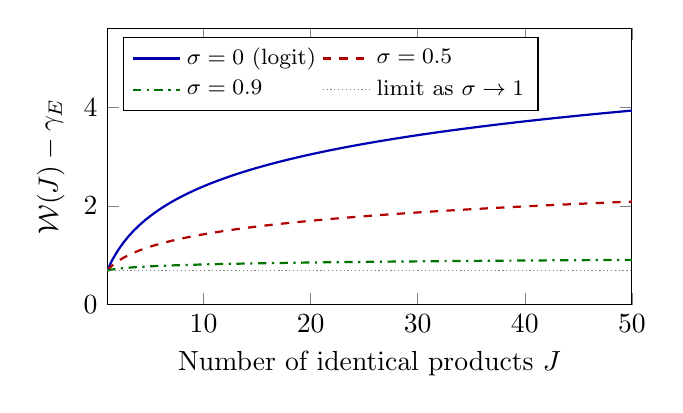
\begin{tikzpicture}
\begin{axis}[width=0.68\textwidth, height=0.42\textwidth,
  xlabel={Number of identical products $J$}, ylabel={$\mathcal{W}(J) - \gamma_E$},
  xmin=1, xmax=50, ymin=0, ymax=5.6, domain=1:50, samples=99,
  legend style={at={(0.03,0.97)}, anchor=north west, font=\footnotesize}, legend columns=2,
  legend cell align=left,
  every axis plot/.append style={thick}]
\addplot[blue!70!black] {ln(1 + x)};
\addlegendentry{$\sigma = 0$ (logit)}
\addplot[red!70!black, dashed] {ln(1 + x^0.5)};
\addlegendentry{$\sigma = 0.5$}
\addplot[green!45!black, dashdotted] {ln(1 + x^0.1)};
\addlegendentry{$\sigma = 0.9$}
\addplot[gray, thin, densely dotted] {ln(2)};
\addlegendentry{limit as $\sigma \rightarrow 1$}
\end{axis}
\end{tikzpicture}
\caption{Expected maximum utility with $J$ identical products in one nest, from \eqref{eq:07-clones} with mean
utility $\delta = 0$ and an outside good. Under the logit the value of variety grows like $\ln J$. The nested logit
slows the growth to $(1-\sigma)\ln J$, and only the limit $\sigma \to 1$ values fifty copies like one product.}
\label{fig:07-clones}
\end{figure}

\casehead{New goods and infinite virtual prices}
The \emph{virtual price} of a product is the price at which its demand falls to zero. Valuing a new good amounts to
integrating its demand curve from the virtual price down to the actual price \citep{Hausman1997}. In the logit the
share of $j$ is positive at every finite price, so the virtual price is infinite. The welfare integral still converges,
because the logit share decays exponentially in price. By the Roy identity of \cref{prop:07-logsum}, and because
$\Lambda$ approaches its value without $j$ as $p_j \to \infty$,
\begin{equation}\label{eq:07-newgood}
\int_{p_j}^{\infty}s_j(t)\,\dd t = \frac{1}{\alpha}\ln\frac{\Lambda^{\text{with } j}}{\Lambda^{\text{without } j}}
= -\frac{1}{\alpha}\ln\big(1 - s_j\big) ,
\end{equation}
where $s_j$ is the share of the new product after its introduction. This is \eqref{eq:07-removal-logit} with the sign
reversed. For small shares the value is close to $\frac{s_j}{\alpha}$. The logit markup of a single-product firm is
$\frac{1}{\alpha(1-s_j)}$, so its variable profit per consumer is $\frac{s_j}{\alpha(1-s_j)}$. The ratio of consumer
surplus to variable profit is $-\frac{(1-s_j)\ln(1-s_j)}{s_j}$, which lies below one and tends to one as $s_j \to 0$. In
the logit, a small new product therefore creates roughly as much consumer surplus as variable profit, whatever its
characteristics.

This mechanical link is the core of the critique of logit welfare analysis. \citet[p.~230]{Hausman1997} writes that the
IIA problem ``typically leads to a vast overestimate of the consumer's surplus from a new good.'' The reason, he adds,
is that ``the model does not incorporate sufficiently the similarities to existing goods.'' The CES demand system has the same feature: an
infinite virtual price and a gain from every new variety (\cref{ch:aids,ch:newgoods}). Nesting the new product with
close substitutes lowers its value through \eqref{eq:07-removal-nl}. Random coefficients let the data decide how
close the new product is to existing ones. \Citet{Trajtenberg1989} values CT scanners with a nested multinomial
logit, and \citet{Petrin2002} contrasts logit and random coefficients valuations of the minivan. \Cref{ch:newgoods}
covers both.

\subsection{Caveats}\label{sec:07-welfare-caveats}

\casehead{Income effects}
The log-sum formula relies on a constant marginal utility of income. Many applications instead use
$\alpha\ln(y_i - p_j)$, as \citet{BerryLevinsohnPakes1995} do, so that richer consumers are less price sensitive.
The marginal utility of income then varies across consumers and across the products they buy. Expected maximum
utility no longer converts into dollars by division by a constant, and the expected compensating variation must be
computed consumer by consumer. For each simulated consumer we draw the random coefficients and the shocks $e_{ij}$,
and we hold the draw fixed across the two choice sets. We then solve for the income change that makes her realized
maximum utility after the change equal to the one before it, and we average across consumers. Under the log form
each such compensation has a closed form (\cref{sec:10-petrin-cv}). The computation reuses the random coefficient
draws of the estimator of \cref{ch:blp} and adds draws of the shocks.

A tempting shortcut integrates out the shocks first. For each draw of the random coefficients, it solves for the
income change that restores expected maximum utility. The result is an ex ante compensation, paid before the shocks
are known, and it generally differs from the mean compensating variation. Take a consumer with income $y$ who has
only the outside good, with utility $\ln y + \epsilon_{i0}$, and add a free alternative with utility $\ln y +
\epsilon_{i1}$. The expected maximum of two independent standard type-I extreme value shocks exceeds that of one by
$\ln 2$, so restoring expected maximum utility requires $\ln(y - C) + \ln 2 = \ln y$, or $C = \frac{y}{2}$. The
realized compensation is $y\big[1 - e^{\epsilon_{i0} - \max(\epsilon_{i0}, \epsilon_{i1})}\big]$. Because
$\epsilon_{i1} - \epsilon_{i0}$ is logistic, the mean realized compensation is $(1 - \ln 2)y \approx 0.307y$. The two measures coincide when
utility is linear in income, so the log-sum formula needs no such distinction.

\casehead{What the shocks mean}
The welfare formulas treat the shocks $\epsilon_{ij}$ as tastes that consumers enjoy. \Cref{sec:07-logit-setup}
listed other readings, from unobserved characteristics to measurement error and mistakes. If the shocks are
mistakes, the log-sum counts them as real utility and overstates welfare. Under every reading, the model gives each
product its own dimension of taste and a group of consumers who prefer it. The result is positive shares, markups
of at least $\frac{1-\sigma}{\alpha}$, and positive value from every added product. This is the ``too many
characteristics'' problem. It biases estimated markups and the value of new goods upward, and it keeps products with zero
sales out of the direct inversion of observed shares. \Cref{sec:07-limits-epsilon} examines its consequences and the remedies proposed
in the literature.

\casehead{Scale and the outside good}
Welfare in dollars does not depend on the scale normalization of the shocks. Scaling all shocks by a constant scales
$\alpha$ and the mean utilities by the same constant, and the ratio in \eqref{eq:07-dcs} is unchanged. Welfare does
depend on the definition of the outside good and of market size, through \eqref{eq:07-dcs-s0}. A study that doubles the
assumed number of potential buyers changes $s_0$ in every market and changes every welfare number with it.
